\documentclass[border=10pt]{standalone}

\usepackage{tikz}
\usepackage{tikzsymbols}
\usetikzlibrary{calc,patterns,shapes.geometric}

\def\centerarc[#1](#2)(#3:#4:#5){\draw[#1] ($(#2)+({#5*cos(#3)},{#5*sin(#3)})$) arc (#3:#4:#5);}

\begin{document}
	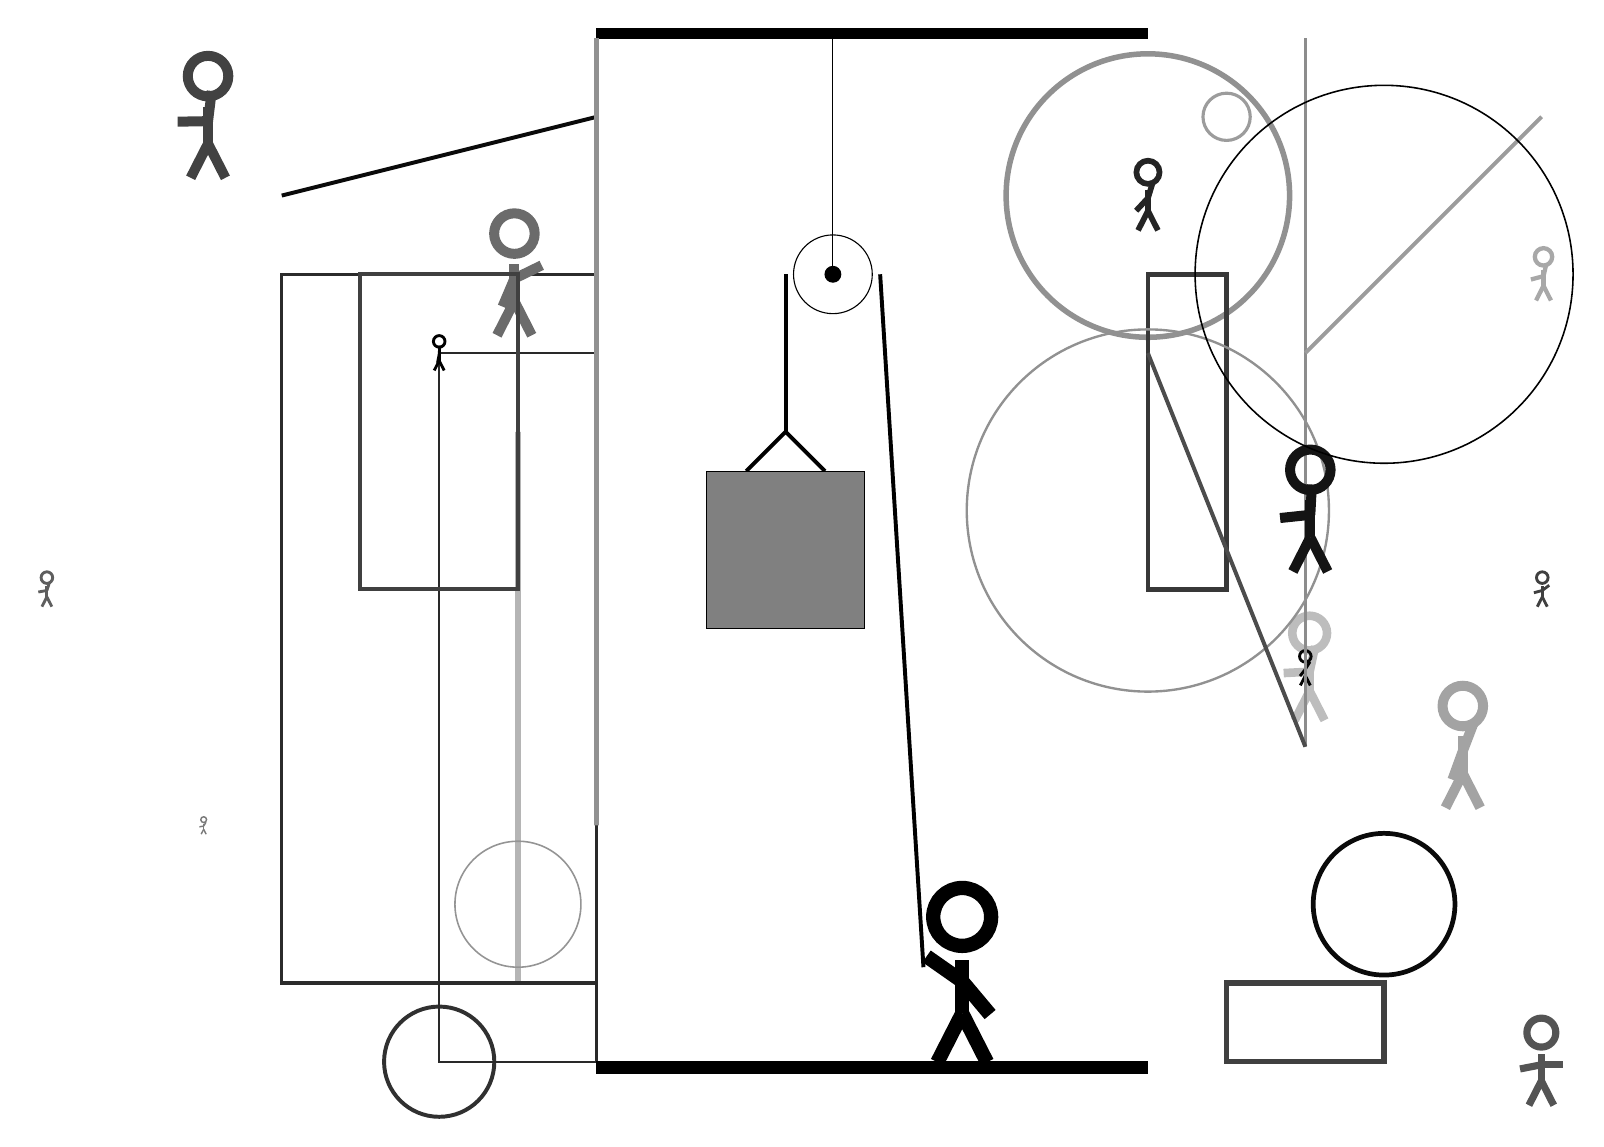
\begin{tikzpicture}
		%%%%% START %%%%%
		
		\draw[fill=black] (-2, 10) rectangle (5, 10.125);
		
		\draw (1, 7) circle (0.5);
		\draw[fill=black] (1, 7) circle (0.1);
		\draw (1, 10) -- (1, 7);
		
		\draw[line width=0.5mm] (-0.1, 4.5) -- (0.4, 5.0) -- (0.9, 4.5);
		\draw[fill=black!50] (-0.6, 4.5) rectangle (1.4, 2.5);
		
		\draw[line width=0.5mm] (0.4, 7) -- (0.4, 5.0);
		\centerarc[line width=0.5mm](1, 7)(0:180:0.6);
		\draw[line width=0.5mm](1.6, 7) -- (2.15, -1.8);
		
		\node at (2.6, -1.9) {\Strichmaxerl[10][-35][-50]};
		
		\node[line width=0.5mm, color=black!67] at (10, -3) {\Strichmaxerl[5][11][0]};
		
		\node[line width=0.4mm, color=black!26] at (7, 2) {\Strichmaxerl[6][3][78]};
		\draw[line width=0.7mm, color=black!29] (-3, -2) rectangle (-3, 5);
		\draw [line width=0.4mm, color=black!39](6, 9) circle (0.3);
		\node[line width=0.2mm, color=black!98] at (7, 2) {\Strichmaxerl[2][52][58]};
		\draw [line width=0.6mm, color=black!96](8, -1) circle (0.9);
		
		\draw[line width=0.4mm, color=black!90] (-2, 8) rectangle (-2, 4);
		
		\draw [line width=0.7mm, color=black!43](5, 8) circle (1.8);
		\node[line width=0.4mm, color=black!52] at (-7, 0) {\Strichmaxerl[1][10][59]};
		\draw [line width=0.5mm, color=black!81](-4, -3) circle (0.7);
		\draw[line width=0.5mm, color=black!96](-6, 8) -- (-2, 9);
		\draw[line width=0.7mm, color=black!58] (-2, 10) rectangle (-2, 9);
		\draw[line width=0.3mm, color=black!45] (7, 10) rectangle (7, 1);
		
		\node[line width=0.4mm, color=black!36] at (9, 1) {\Strichmaxerl[7][70][69]};
		\draw[line width=0.6mm, color=black!78] (5, 7) rectangle (6, 3);
		\node[line width=0.4mm, color=black!63] at (-9, 3) {\Strichmaxerl[2][10][72]};
		
		\draw [line width=0.3mm, color=black!43](5, 4) circle (2.3);
		\draw[line width=0.4mm, color=black!83] (-2, 7) rectangle (-6, -2);
		\node[line width=0.7mm, color=black!58] at (-3, 7) {\Strichmaxerl[7][67][26]};
		\node[line width=0.4mm, color=black!92] at (7, 4) {\Strichmaxerl[7][6][87]};
		\draw[line width=0.3mm, color=black!84] (-2, -3) rectangle (-4, 6);
		\draw[line width=0.5mm, color=black!39](10, 9) -- (7, 6);
		\node[line width=0.6mm, color=black!75] at (10, 3) {\Strichmaxerl[2][15][37]};
		\draw[line width=0.5mm, color=black!70](5, 6) -- (7, 1);
		\node[line width=0.4mm, color=black!34] at (10, 7) {\Strichmaxerl[3][15][77]};
		
		\node[line width=0.2mm, color=black!86] at (5, 8) {\Strichmaxerl[4][47][73]};
		
		\node[line width=0.3mm, color=black!100] at (-4, 6) {\Strichmaxerl[2][79][86]};
		\draw[line width=0.7mm, color=black!43] (-2, 10) rectangle (-2, 0);
		\draw[line width=0.7mm, color=black!75] (6, -2) rectangle (8, -3);
		\draw[line width=0.5mm, color=black!75] (-3, 3) rectangle (-5, 7);
		\draw [line width=0.2mm, color=black!42](-3, -1) circle (0.8);
		
		\node[line width=0.6mm, color=black!74] at (-7, 9) {\Strichmaxerl[7][1][83]};
		\draw [line width=0.2mm, color=black!100](8, 7) circle (2.4);
		
		\draw[fill=black] (-2, -3) rectangle (5, -3.15);
		
		%%%%% END %%%%%
	\end{tikzpicture}
\end{document}